\documentclass[calculator,datasheet,handbook,solutions]{exam}
% The full list of class options are
% calculator : Allows approved calculator use.
% datasheet : Adds a note that data sheet are attached to the exam.
% handbook : Allows the use of the engineering handbook.
% resit : Adds the resit markings to the paper.
% sample : Adds conspicuous SAMPLE markings to the paper
% solutions : Uses the contents of \solution commands (and \solmarks) to generate a solution file

\usepackage{array}
\usepackage{multirow}
\usepackage{pdfpages}
\usepackage[hidelinks]{hyperref}

\examtime{2~pm -- 5~pm}%
\examdate{13}{12}{2016}%
\examformat{Candidates should attempt \textit{all} questions.}

\newtoggle{3030paper}

%This changes the mode from EX3030 to EM40JN
\toggletrue{3030paper}
%\togglefalse{3030paper}

\iftoggle{3030paper}{
  \coursecode{EX3030}%
  \coursetitle{Heat, Mass, \& Momentum Transfer}%
}{
  \coursecode{EM40JN}%
  \coursetitle{Heat and Momentum Transfer}%
}

\begin{document}
%%%%%%%%%%%%%%%%%%%%%%%%%%%%%%%%%%%%%%%%%%%%%%%%%%%%%%%%%%%%%%%%%%%%%%%%%%%%%%%% 
%%%%%%%%%%%%%%%%%%%%%%%%%%%%%%%%%%%%%%%%%%%%%%%%%%%%%%%%%%%%%%%%%%%%%%%%%%%%%%%%

\begin{question}
  \begin{enumerate}[a)]
     \item In a binary geothermal power plant, the working fluid isobutane is condensed by air in a condenser at 75$^{\circ}$C $\left(h_{\text{fg}}=\text{ 255.7 kJ/kg}\right)$ at a rate of 2.7 kg/s. Air enters the condenser at 21$^{\circ}$C and leaves at 28$^{\circ}$C. The heat transfer surface area based on the isobutane side is 24 m$^{2}$. Determine the mass flow rate of air (in kg/s) and the overall heat transfer coefficient $\left(\text{in W/}\left(\text{m}^{2}.^{\circ}\text{C}\right)\right)$. Assume that: (i) there is no heat losses across the border of the condenser and (ii)etrams of isobutane and air are counterflow. Given the specific heat capacity of air of 1005 J/$\left(\text{kg.}^{\circ}\text{C}\right)$.\marks{8}
     \solution{The mass flow rate of air can be obtained from the energy balance across the borders assuming no heat losses,\solmarks{1}
           \begin{displaymath}
                 \left|\dot{Q}_{\text{air}}\right| = \left|\dot{Q}_{\text{iC4}}\right|
           \end{displaymath}
The rate of heat transfer during condensation of isobtane can be determined by\solmarks{1}
         \begin{displaymath}
            \dot{Q}_{\text{iC4}} = \left(\dot{m}h_{fg}\right)_{\text{iC4}} = 690.39 \text{ kJ/s}
         \end{displaymath}
         The mass flow rate of air is determined from\solmarks{2}
         \begin{displaymath}
            \dot{Q}_{\text{air}} = \left[\dot{m}C_{p}\left(T_{\text{out}}-T_{\text{in}}\right)\right]_{\text{air}}\;\;\;\Rightarrow \dot{m}_{\text{air}} = 98.14\text{ kg/s}
         \end{displaymath}
The overall heat transfer coefficient can be obtained by the LMTD method,
          \begin{displaymath}
             \dot{Q} = U A_{s} \Delta T_{\text{lm}}
          \end{displaymath}
           where $\Delta T_{\text{lm}}$ is given by
           \begin{displaymath}
              \Delta T_{\text{lm}} = \frac{\Delta T_{1}-\Delta T_{2}}{\ln{\frac{\Delta T_{1}}{\Delta T_{2}}}}
           \end{displaymath}
           where\solmarks{2}
         \begin{displaymath}
               \begin{cases}
                   \Delta T_{1} = T_{\text{h,in}}-T_{\text{c,out}} = 54^{\circ}\text{C} \\
                   \Delta T_{2} = T_{\text{h,out}}-T_{\text{c,in}} = 47^{\circ}\text{C} \\
               \end{cases} 
         \end{displaymath}
$\Delta T_{\text{lm}}$ can be obtained as 50.4$^{\circ}\text{C}$\solmarks{1}. And the overall heat transfer coefficient is,\solmarks{1}
          \begin{displaymath}
             \dot{Q} = U A_{s} \Delta T_{\text{lm}}\;\;\Rightarrow U = 571 \text{ W/}\left(\text{m}^{2}.^{\circ}\text{C}\right)
          \end{displaymath}
}
    \item A long rod of 60 mm diameter and thermophysical properties $\rho=$ 8000 kg/m$^{3}$, $C_{p}=$ 500 J/(kg.K), and $k=$ 50 W/(m.K) is initially at a uniform temperature and is heated in a forced convection furnace maintained at 750 K. The convection coefficient is estimated to be 1000 W/(m$^{2}$.K). Calculate the centerline temperature of the rod when the surface temperature is 550 K.\marks{12}
   \solution{ Assuming that the Fourier number for this problem is larger than 0.2, we can use the 1D analytical solution for the transient conductive equation,\solmarks{1}
        \begin{displaymath}
           \theta_{\text{cyl}} = \frac{T(r,t)-T_{\infty}}{T_{i}-T_{\infty}}= A_{1}e^{-\lambda_{1}^{2}\tau}\mathbf{J_{0}}\left(\frac{\lambda_{1}r}{r_{0}}\right)
        \end{displaymath}
and at the centre of the geometry,\solmarks{2}
        \begin{displaymath}
           \theta_{\text{cyl}} = \frac{T(0,t)-T_{\infty}}{T_{i}-T_{\infty}}= A_{1}e^{-\lambda_{1}^{2}\tau}
        \end{displaymath}
We need to obtain $T(0,t)$ at time $t=t_{i}$ such that $T\left(r_{0},t_{i}\right) =$ 500 K. Merging both equations,\solmarks{3}
        \begin{displaymath}
           \frac{T(r_{0},t_{i})-T_{\infty}}{T_{i}-T_{\infty}} = \frac{T(0,t_{i})-T_{\infty}}{T_{i}-T_{\infty}}\mathbf{J_{0}}\left(\frac{\lambda_{1}r_{0}}{r_{0}}\right)
        \end{displaymath}
In order to solve this expression, $\mathbf{J_{0}}\left(\frac{\lambda_{1}r}{r_{0}}\right)$ and $\lambda_{1}$ need to be obtained from the Table of coefficients for the approximate solution of the transient 1D heat conduction based on,\solmarks{3}
       \begin{displaymath}
           Bi = \frac{h r_{0}}{\kappa} = 0.60 \;\;\Rightarrow \;\; \lambda_{1} = 1.0184\;\;\text{ and }\;\; \mathbf{J_{0}}\left(\frac{\lambda_{1}r_{0}}{r_{0}}\right) = \mathbf{J_{0}}\left(\lambda_{1}\right) = 0.7571
       \end{displaymath} 
Replacing $\mathbf{J_{0}}$ in the merged equation, \solmarks{3}
       \begin{displaymath}
           (550-750) = \left[T\left(0,t_{i}\right)-750\right] \times 0.7571 \;\;\Rightarrow T\left(0,t_{i}\right) = 485.83\text{ K}
       \end{displaymath} 
    
    




}

  \end{enumerate}
\end{question}

\pagebreak

%%%%%%%%%%%%%%%%%%%%%%%%%%%%%%%%%%%%%%%%%%%%%%%%%%%%%%%%%%%%%%%%%%%%%%%%%%%%%%%%%%%%%%%%%%%%%%%%%%%%%%%%%%%%%% 
%%%%%%%%%%%%%%%%%%%%%%%%%%%%%%%%%%%%%%%%%%%%%%%%%%%%%%%%%%%%%%%%%%%%%%%%%%%%%%%%%%%%%%%%%%%%%%%%%%%%%%%%%%%%%% 
\begin{datasheet}
{\bf General balance equations:}
\begin{align}
  \frac{\partial\rho}{\partial t} &= -\nabla \cdot \rho\,\bm{v}\label{eq:continuity} & \text{(Mass/Continuity)}\\
  \frac{\partial C_A}{\partial t} &= -\nabla\cdot\bm{N}_{A} + \sigma_A& \text{(Species)}\\
  \rho \frac{\partial\bm{v}}{\partial t} &= -\rho\,\bm{v}\cdot\nabla
  \bm{v}
  - \nabla\cdot\bm{\tau} - \nabla\,p + \rho\,\bm{g}\label{eq:momentumbalance} & \text{(Momentum)}\\
  \rho\,C_p\frac{\partial T}{\partial t} &= -\rho\,C_p\,\bm{v}
  \cdot\nabla\,T - \nabla\cdot\bm{q} - \bm{\tau}:\nabla\,\bm{v} -
  p\,\nabla\cdot\bm{v} +\sigma_{energy}\label{eq:energybalance} &
  \text{(Heat/Energy)}
\end{align}

In Cartesian coordinate systems, $\nabla$ can be treated as a vector of
derivatives. In curvelinear coordinate systems, the directions
$\hat{\bm{r}}$, $\hat{\bm{\theta}}$, and $\hat{\bm{\phi}}$ depend on
the position. For convenience in these systems, look-up tables are
provided for common terms involving $\nabla$.

\vspace{\baselineskip}
{\bf Cartesian coordinates} (with index notation examples)\\
where $s$ is a scalar, $\bm{v}$ is a vector, and $\bm{\tau}$ is a tensor.
\begin{align*}
  \nabla s = \nabla_i s &= \left[\frac{\partial\,s}{\partial x},\,
  \frac{\partial\,s}{\partial y},\, \frac{\partial\,s}{\partial z}\right]
  \\
  \nabla^2 s = \nabla_i\nabla_i s &=\frac{\partial^2\,s}{\partial x^2} +
  \frac{\partial^2\,s}{\partial y^2}+ \frac{\partial^2\,s}{\partial z^2}
  \\
  \nabla\cdot\bm{v} =\nabla_i v_i &= \frac{\partial\,v_x}{\partial x} +
  \frac{\partial\,v_y}{\partial y}+ \frac{\partial\,v_z}{\partial z}
  \\
  \nabla \cdot \bm{\tau} &= \nabla_i\, \tau_{ij}
  \\
  \left[\nabla \cdot \bm{\tau}\right]_x &= \frac{\partial\,\tau_{xx}}{\partial x} +
  \frac{\partial\, \tau_{yx}}{\partial y} + \frac{\partial\, \tau_{zx}}{\partial z}
  \\
  \left[\nabla \cdot \bm{\tau}\right]_y &= \frac{\partial\,\tau_{xy}}{\partial x} +
  \frac{\partial\, \tau_{yy}}{\partial y} + \frac{\partial\, \tau_{zy}}{\partial z}
  \\
  \left[\nabla \cdot \bm{\tau}\right]_z &= \frac{\partial\,\tau_{xz}}{\partial x} +
  \frac{\partial\, \tau_{yz}}{\partial y} + \frac{\partial\, \tau_{zz}}{\partial z}
  \\
  \bm{v}\cdot \nabla \bm{v} &= v_i\,\nabla_i\,v_j
  \\
  \left[\bm{v}\cdot \nabla \bm{v}\right]_x &= v_x\frac{\partial\,v_x}{\partial x} + v_y\frac{\partial\,v_x}{\partial y} +v_z\frac{\partial\,v_x}{\partial z}
  \\
  \left[\bm{v}\cdot \nabla \bm{v}\right]_y &= v_x\frac{\partial\,v_y}{\partial x} + v_y\frac{\partial\,v_y}{\partial y} +v_z\frac{\partial\,v_y}{\partial z}
  \\
  \left[\bm{v}\cdot \nabla \bm{v}\right]_z &= v_x\frac{\partial\,v_z}{\partial x} + v_y\frac{\partial\,v_z}{\partial y} +v_z\frac{\partial\,v_z}{\partial z}
\end{align*}

\pagebreak
{\bf Cylindrical coordinates}\\
where $s$ is a scalar, $\bm{v}$ is a vector, and $\bm{\tau}$ is a
tensor. All expressions involving $\bm{\tau}$ are for symmetrical
$\bm{\tau}$ only.
\begin{align*}
  \nabla s &= \left[\frac{\partial\,s}{\partial r},\,
    \frac{1}{r}\frac{\partial\,s}{\partial \theta},\,
    \frac{\partial\,s}{\partial z}\right]
  \\
  \nabla^2 s &=\frac{1}{r}\frac{\partial}{\partial
    r}\left(r\frac{\partial s}{\partial r}\right) +
  \frac{1}{r^2}\frac{\partial^2\,s}{\partial \theta^2}+
  \frac{\partial^2\,s}{\partial z^2}
  \\
  \nabla\cdot\bm{v} &= \frac{1}{r}\frac{\partial}{\partial r}\left(r\,
    v_r\right) + \frac{1}{r}\frac{\partial\,v_\theta}{\partial
    \theta}+ \frac{\partial\,v_z}{\partial z}
  \\
  \left[\nabla \cdot \bm{\tau}\right]_r &=
  \frac{1}{r}\frac{\partial}{\partial r}\left(r\,\tau_{rr}\right) +
  \frac{1}{r}\frac{\partial\, \tau_{r\theta}}{\partial \theta} -
  \frac{1}{r} \tau_{\theta\theta} + \frac{\partial\,
    \tau_{rz}}{\partial z}
  \\
  \left[\nabla \cdot \bm{\tau}\right]_\theta &=
  \frac{1}{r}\frac{\partial \tau_{\theta\theta}}{\partial \theta} +
  \frac{\partial\, \tau_{r\theta}}{\partial r} + \frac{2}{r}
  \tau_{r\theta} + \frac{\partial\, \tau_{\theta z}}{\partial z}
  \\
  \left[\nabla \cdot \bm{\tau}\right]_z &= \frac{1}{r}\frac{\partial
  }{\partial r}\left(r\,\tau_{rz}\right) + \frac{1}{r}\frac{\partial
    \tau_{\theta z}}{\partial\theta} + \frac{\partial\, \tau_{z
      z}}{\partial z}
  \\
  \left[\bm{v}\cdot \nabla \bm{v}\right]_r &= v_r \frac{\partial
    v_r}{\partial r} + \frac{v_\theta}{r}\frac{\partial v_r}{\partial
    \theta} - \frac{v_\theta^2}{r}+v_z\frac{\partial v_r}{\partial z}
  \\
  \left[\bm{v}\cdot \nabla \bm{v}\right]_\theta &=
  v_r \frac{\partial v_\theta}{\partial r} + \frac{v_\theta}{r}\frac{\partial v_\theta}{\partial \theta} + \frac{v_r\,v_\theta}{r} + v_z \frac{\partial v_\theta}{\partial z}
  \\
  \left[\bm{v}\cdot \nabla \bm{v}\right]_z &=
  v_r \frac{\partial v_z}{\partial r} + \frac{v_\theta}{r}\frac{\partial v_z}{\partial \theta}+v_z \frac{\partial v_z}{\partial z}
\end{align*}
{\bf Spherical coordinates}\\
where $s$ is a scalar, $\bm{v}$ is a vector, and $\bm{\tau}$ is a
tensor. All expressions involving $\bm{\tau}$ are for symmetrical
$\bm{\tau}$ only.
\begin{align*}
  \nabla s &= \left[\frac{\partial\,s}{\partial r},\,
    \frac{1}{r}\frac{\partial\,s}{\partial \theta},\,
    \frac{1}{r\,\sin\theta}\frac{\partial\,s}{\partial \phi}\right]
  \\
  \nabla^2 s &=\frac{1}{r^2}\frac{\partial}{\partial r}\left(r^2
    \frac{\partial s}{\partial r}\right) +
  \frac{1}{r^2\sin\theta}\frac{\partial}{\partial
    \theta}\left(\sin\theta \frac{\partial s}{\partial \theta}\right)+
  \frac{1}{r^2 \sin^2\theta}\frac{\partial^2\,s}{\partial \phi^2}
  \\
  \nabla\cdot\bm{v} &= \frac{1}{r^2}\frac{\partial}{\partial
    r}\left(r^2\, v_r\right) +
  \frac{1}{r\sin\theta}\frac{\partial}{\partial
    \theta}\left(v_\theta\sin\theta\right)+
  \frac{1}{r\sin\theta}\frac{\partial\,v_\phi}{\partial \phi}
  \\
  \left[\nabla \cdot \bm{\tau}\right]_r &=
  \frac{1}{r^2}\frac{\partial}{\partial r}\left(r^2\,\tau_{rr}\right)
  + \frac{1}{r\sin\theta}\frac{\partial}{\partial
    \theta}\left(\tau_{r\theta}\sin\theta\right)
  +\frac{1}{r\sin\theta}\frac{\partial\, \tau_{r\phi}}{\partial \phi}
  - \frac{\tau_{\theta\theta}+\tau_{\phi\phi}}{r}
  \\
  \left[\nabla \cdot \bm{\tau}\right]_\theta &=
  \frac{1}{r^2}\frac{\partial}{\partial
    r}\left(r^2\,\tau_{r\theta}\right) +
  \frac{1}{r\sin\theta}\frac{\partial}{\partial
    \theta}\left(\tau_{\theta\theta}\sin\theta\right)
  +\frac{1}{r\sin\theta}\frac{\partial\, \tau_{\theta\phi}}{\partial
    \phi} + \frac{\tau_{r\theta}}{r} -
  \frac{\cot\theta}{r}\tau_{\phi\phi}
  \\
  \left[\nabla \cdot \bm{\tau}\right]_\phi &=
  \frac{1}{r^2}\frac{\partial}{\partial
    r}\left(r^2\,\tau_{r\phi}\right) + \frac{1}{r}\frac{\partial
    \tau_{\theta\phi}}{\partial \theta}
  +\frac{1}{r\sin\theta}\frac{\partial\, \tau_{\phi\phi}}{\partial
    \phi} + \frac{\tau_{r\theta}}{r} +
  \frac{2\cot\theta}{r}\tau_{\theta\phi}
  \\
  \left[\bm{v}\cdot \nabla \bm{v}\right]_r &= v_r \frac{\partial
    v_r}{\partial r} + \frac{v_\theta}{r}\frac{\partial v_r}{\partial
    \theta} + \frac{v_\phi}{r\sin\theta}\frac{\partial v_r}{\partial
    \phi}-\frac{v_\theta^2+v_\phi^2}{r}
  \\
  \left[\bm{v}\cdot \nabla \bm{v}\right]_\theta &= v_r \frac{\partial
    v_\theta}{\partial r} + \frac{v_\theta}{r}\frac{\partial v_\theta}{\partial
    \theta} + \frac{v_\phi}{r\sin\theta}\frac{\partial v_\theta}{\partial
    \phi}+\frac{v_r\,v_\theta -v_\phi^2\cot\theta}{r}
  \\
  \left[\bm{v}\cdot \nabla \bm{v}\right]_\phi &= v_r \frac{\partial
    v_\phi}{\partial r} + \frac{v_\theta}{r}\frac{\partial v_\phi}{\partial
    \theta} + \frac{v_\phi}{r\sin\theta}\frac{\partial v_\phi}{\partial
    \phi}+\frac{v_r\,v_\phi +v_\theta\,v_\phi\cot\theta}{r}
\end{align*}
\begin{table}[h!]\label{tab:constitutive}
  {\hspace{-25pt}\setlength{\extrarowheight}{5pt}%
    \begin{tabular}{|r|c|r|c|r|c|}
      \hline
      \multicolumn{2}{|c|}{Rectangular} & \multicolumn{2}{c|}{Cylindrical} & \multicolumn{2}{c|}{Spherical}
      \\\hline\hline
      $q_x$ & $-k\frac{\partial T}{\partial x}$ &
      $q_r$ & $-k\frac{\partial T}{\partial r}$ &
      $q_r$ & $-k\frac{\partial T}{\partial r}$
      \\[5pt]\hline
      $q_y$ & $-k\frac{\partial T}{\partial y}$ &
      $q_\theta$ & $-k\frac{1}{r}\frac{\partial T}{\partial \theta}$ &
      $q_\theta$ & $-k\frac{1}{r}\frac{\partial T}{\partial \theta}$ 
      \\[5pt]\hline
      $q_z$ & $-k\frac{\partial T}{\partial z}$ &
      $q_z$ & $-k\frac{\partial T}{\partial z}$ & 
      $q_\phi$ & $-k\frac{1}{r\,\sin\theta}\frac{\partial T}{\partial \phi}$
      \\[5pt]\hline
      $\tau_{xx}$
      &$-2\,\mu\frac{\partial v_x}{\partial x} + \mu^B \,\nabla\cdot\bm{v}$
      & $\tau_{rr}$ & $-2\,\mu\frac{\partial v_r}{\partial r} + \mu^B \,\nabla\cdot\bm{v}$
      & $\tau_{rr}$ & $ -2\,\mu\frac{\partial v_r}{\partial r} + \mu^B \,\nabla\cdot\bm{v}$
      \\[5pt]\hline
      $\tau_{yy}$ & $ -2\,\mu\frac{\partial v_y}{\partial y} + \mu^B \,\nabla\cdot\bm{v}$
      & $\tau_{\theta\theta}$ & $-2\,\mu\left(\frac{1}{r}\frac{\partial v_\theta}{\partial\theta}+\frac{v_r}{r}\right) + \mu^B \,\nabla\cdot\bm{v}$
      & $\tau_{\theta\theta}$ & $-2\,\mu\left(\frac{1}{r}\frac{\partial v_\theta}{\partial\theta}+\frac{v_r}{r}\right) + \mu^B \,\nabla\cdot\bm{v}$
      \\[5pt]\hline
      \multirow{2}{*}{$\tau_{zz}$} & \multirow{2}{*}{$-2\,\mu\frac{\partial v_z}{\partial z} + \mu^B \,\nabla\cdot\bm{v}$}
      & \multirow{2}{*}{$\tau_{zz}$} & \multirow{2}{*}{$-2\,\mu\frac{\partial v_z}{\partial z} + \mu^B \,\nabla\cdot\bm{v}$}
      & \multirow{2}{*}{$\tau_{\phi\phi}$} & $-2\,\mu\left(\frac{1}{r\sin\theta}\frac{\partial v_\phi}{\partial \phi} + \frac{v_r+v_\theta\cot\theta}{r}\right)$
      \\
      & & & & & \hfill $+ \mu^B \,\nabla\cdot\bm{v}$
      \\[5pt]\hline
      $\tau_{xy}$ & $-\mu\left(\frac{\partial v_x}{\partial y} +\frac{\partial v_y}{\partial x}\right)$
      & $\tau_{r\theta}$ & $-\mu\left(r\frac{\partial}{\partial r}\left(\frac{v_\theta}{r}\right) +\frac{1}{r}\frac{\partial v_r}{\partial \theta}\right)$
      & $\tau_{r\theta}$ & $-\mu\left(r\frac{\partial}{\partial r}\left(\frac{v_\theta}{r}\right) +\frac{1}{r}\frac{\partial v_r}{\partial \theta}\right)$
      \\[5pt]\hline
      $\tau_{yz}$ & $-\mu\left(\frac{\partial v_y}{\partial z} +\frac{\partial v_z}{\partial y}\right)$
      & $\tau_{\theta z}$ & $-\mu\left(\frac{1}{r}\frac{\partial v_z}{\partial \theta} +\frac{\partial v_\theta}{\partial z}\right)$
      & $\tau_{\theta \phi}$ & $-\mu\left(\frac{\sin\theta}{r}\frac{\partial}{\partial \theta}\left(\frac{v_\phi}{\sin\theta}\right) +\frac{1}{r\sin\theta}\frac{\partial v_\theta}{\partial \phi}\right)$
      \\[5pt]\hline
      $\tau_{xz}$ & $-\mu\left(\frac{\partial v_x}{\partial z} +\frac{\partial v_z}{\partial x}\right)$
      & $\tau_{zr}$ & $-\mu\left(\frac{\partial v_r}{\partial z} +\frac{\partial v_z}{\partial r}\right)$
      & $\tau_{\phi r}$ & $-\mu\left(\frac{1}{r\sin\theta}\frac{\partial v_r}{\partial \phi} +r\frac{\partial}{\partial r}\left(\frac{v_\phi}{r}\right)\right)$
      \\[5pt]\hline
      % \multicolumn{2}{|c|}{$\nabla\cdot\bm{v} = \frac{\partial v_x}{\partial x}+\frac{\partial v_y}{\partial y} +\frac{\partial v_z}{\partial z}$}
      % & \multicolumn{2}{c|}{$\nabla\cdot\bm{v} = \frac{1}{r}\frac{\partial r\,v_r}{\partial r}+\frac{1}{r}\frac{\partial v_\theta}{\partial \theta} +\frac{\partial v_z}{\partial z}$}
      % & \multicolumn{2}{c|}{$\nabla\cdot\bm{v} = \frac{1}{r^2}\frac{\partial r^2\,v_r}{\partial r}+\frac{1}{r\sin\theta}\frac{\partial v_\theta\sin\theta}{\partial \theta} +\frac{1}{r\sin\theta}\frac{\partial v_\phi}{\partial \phi}$}
      % \\[5pt]\hline
    \end{tabular}
  }
  \caption{Fourier's law for the heat flux and Newton's law for the stress in several coordinate systems. Please remember that the stress is symmetric, so $\tau_{ij}=\tau_{ji}$.}
\end{table}

\newpage
{\bf Viscous models:}\\*
Power-Law Fluid:
\begin{align}\label{eq:powerlawfluid}
  \left|\tau_{xy}\right| &= k \left|\frac{\partial v_x}{\partial y}\right|^{n}
\end{align}
Bingham-Plastic Fluid:
\begin{align*}
  \frac{\partial v_x}{\partial y} = \begin{cases}
    -\mu^{-1}\left(\tau_{xy}-\tau_0)\right) & \text{if
      $\tau_{xy} > \tau_0$}
    \\
    0 & \text{if $\tau_{xy} \leq \tau_0$}
  \end{cases}
\end{align*}
{\bf Dimensionless Numbers}\\*
\begin{align}
  \text{Re}&=\frac{\rho\,\left\langle v\right\rangle\,D}{\mu}
  &
  \text{Re}_{H}&=\frac{\rho\,\left\langle v\right\rangle\,D_H}{\mu}
  &
  \text{Re}_{MR}&=-\frac{16\,L\,\rho\left\langle
      v\right\rangle^2}{R\,\Delta p}\label{eq:Reynolds}
\end{align}
The hydraulic diameter is defined as $D_H=4\,A / P_w$.

{\bf Single phase pressure drop calculations in pipes:}\\*
Darcy-Weisbach equation:
\begin{align}
  \frac{\Delta p}{L} = -\frac{C_f\,\rho\left\langle v\right\rangle^2}{R}
\end{align}
where $C_f=16/Re$ for laminar Newtonian flow.  For turbulent flow of
Newtonian fluids in smooth pipes, we have the Blasius correlation:
\begin{align*}
  C_f&=0.079\,\text{Re}^{-1/4} & \text{for $2.5\times10^3<\text{Re}<10^5$ and smooth pipes.}
\end{align*}
Otherwise, you may refer to the Moody diagram.
\begin{figure}[h]
  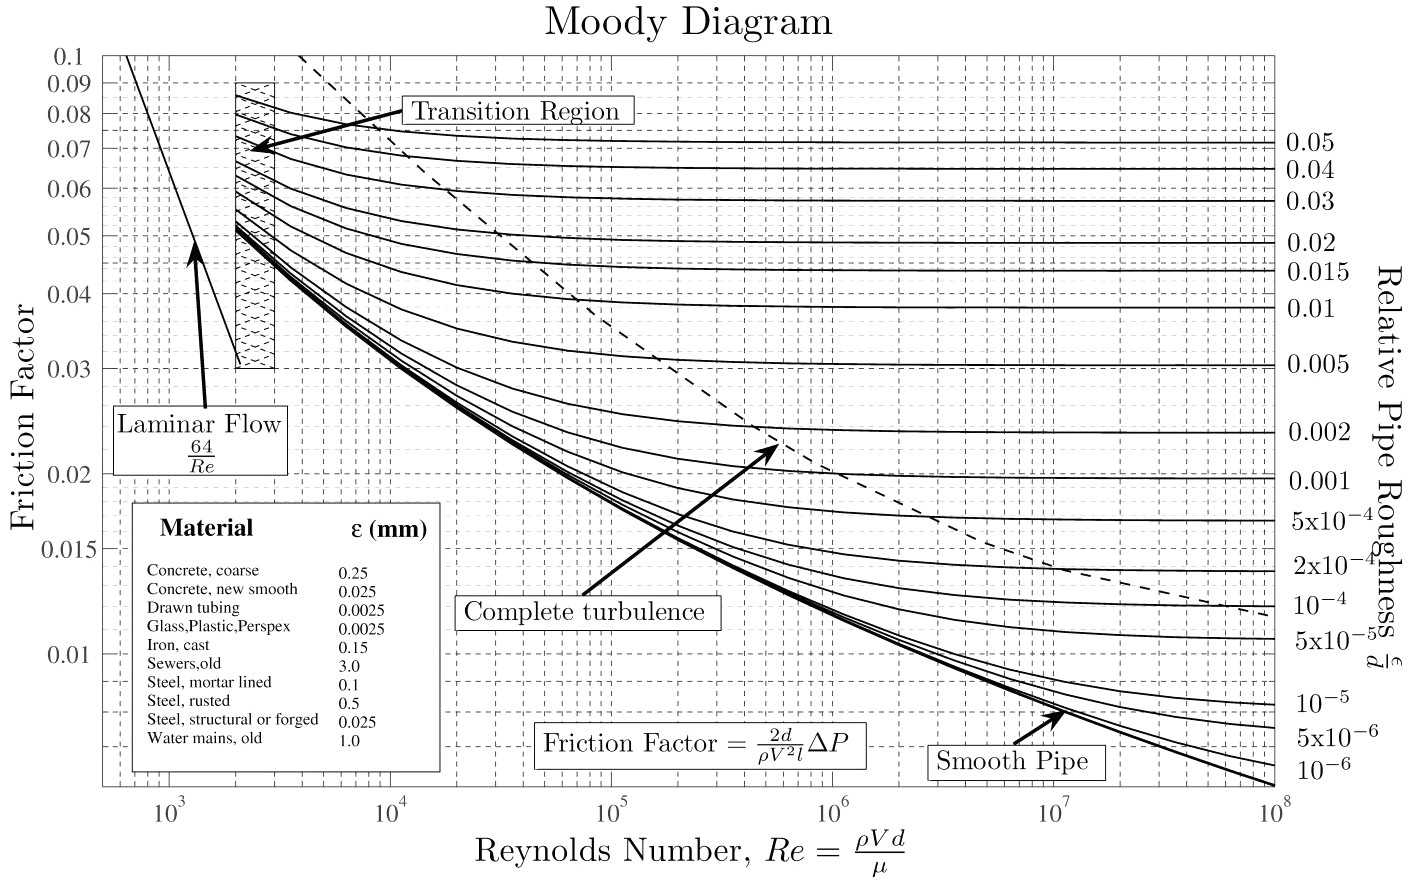
\includegraphics[clip,width=\linewidth]{figures/Moody_diagram}
\end{figure}

Laminar Power-Law fluid:
\begin{align*}
  \dot{V} = \frac{n\,\pi\,R^3}{3\,n+1} \left(\frac{R}{2\,k}\right)^{\frac{1}{n}} \left(-\frac{\Delta p}{L}\right)^{\frac{1}{n}}
\end{align*}
{\bf Two-Phase Flow:}\\*
Lockhart-Martinelli parameter:
\begin{align*}
  X^2=\frac{\Delta p_{liq.-only}}{\Delta p_{gas-only}}
\end{align*}
Pressure drop calculation:
\begin{align*}
  \Delta p_{two-phase} = \Phi^2_{liq.}\,\Delta p_{liq.-only} = \Phi^2_{gas}\,\Delta p_{gas-only}
\end{align*}
Chisholm's relation:
\begin{align*}
  \Phi^2_{gas} &= 1 + c\,X + X^2 &\\
  \Phi^2_{liq.} &= 1 + \frac{c}{X}+\frac{1}{X^2} &
  c &= \begin{cases}
    20& \text{turbulent liquid \& turbulent gas}\\
    12& \text{laminar liquid \& turbulent gas}\\
    10& \text{turbulent liquid \& laminar gas}\\
    5& \text{laminar liquid \& laminar gas}
  \end{cases}
\end{align*}
Farooqi and Richardson expression for liquid hold-up in co-current
flows of Newtonian fluids and air in horizontal pipes:
\begin{align*}
  h &=
  \begin{cases}
    0.186+0.0191\,X & 1 < X < 5\\
    0.143\,X^{0.42} & 5 < X < 50\\
    1/\left(0.97 + 19/X\right) & 50 < X < 500
  \end{cases}
\end{align*}

\begin{figure}[p!]%
  \begin{center}%
    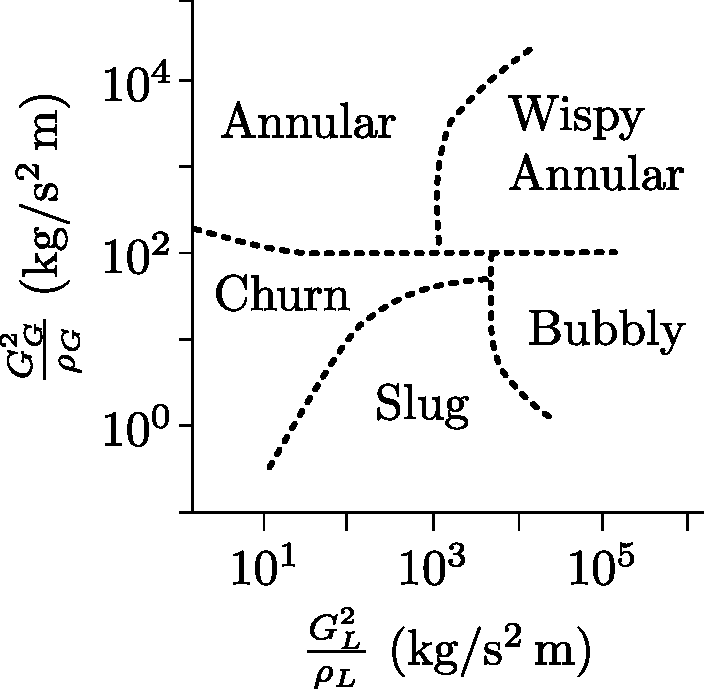
\includegraphics[width=0.65\textwidth,clip]{figures/Hewitt_Taylor}
  \end{center}
  \caption{Hewitt-Taylor flow pattern map for multiphase flows in
    vertical pipes.}
  \begin{center}%
    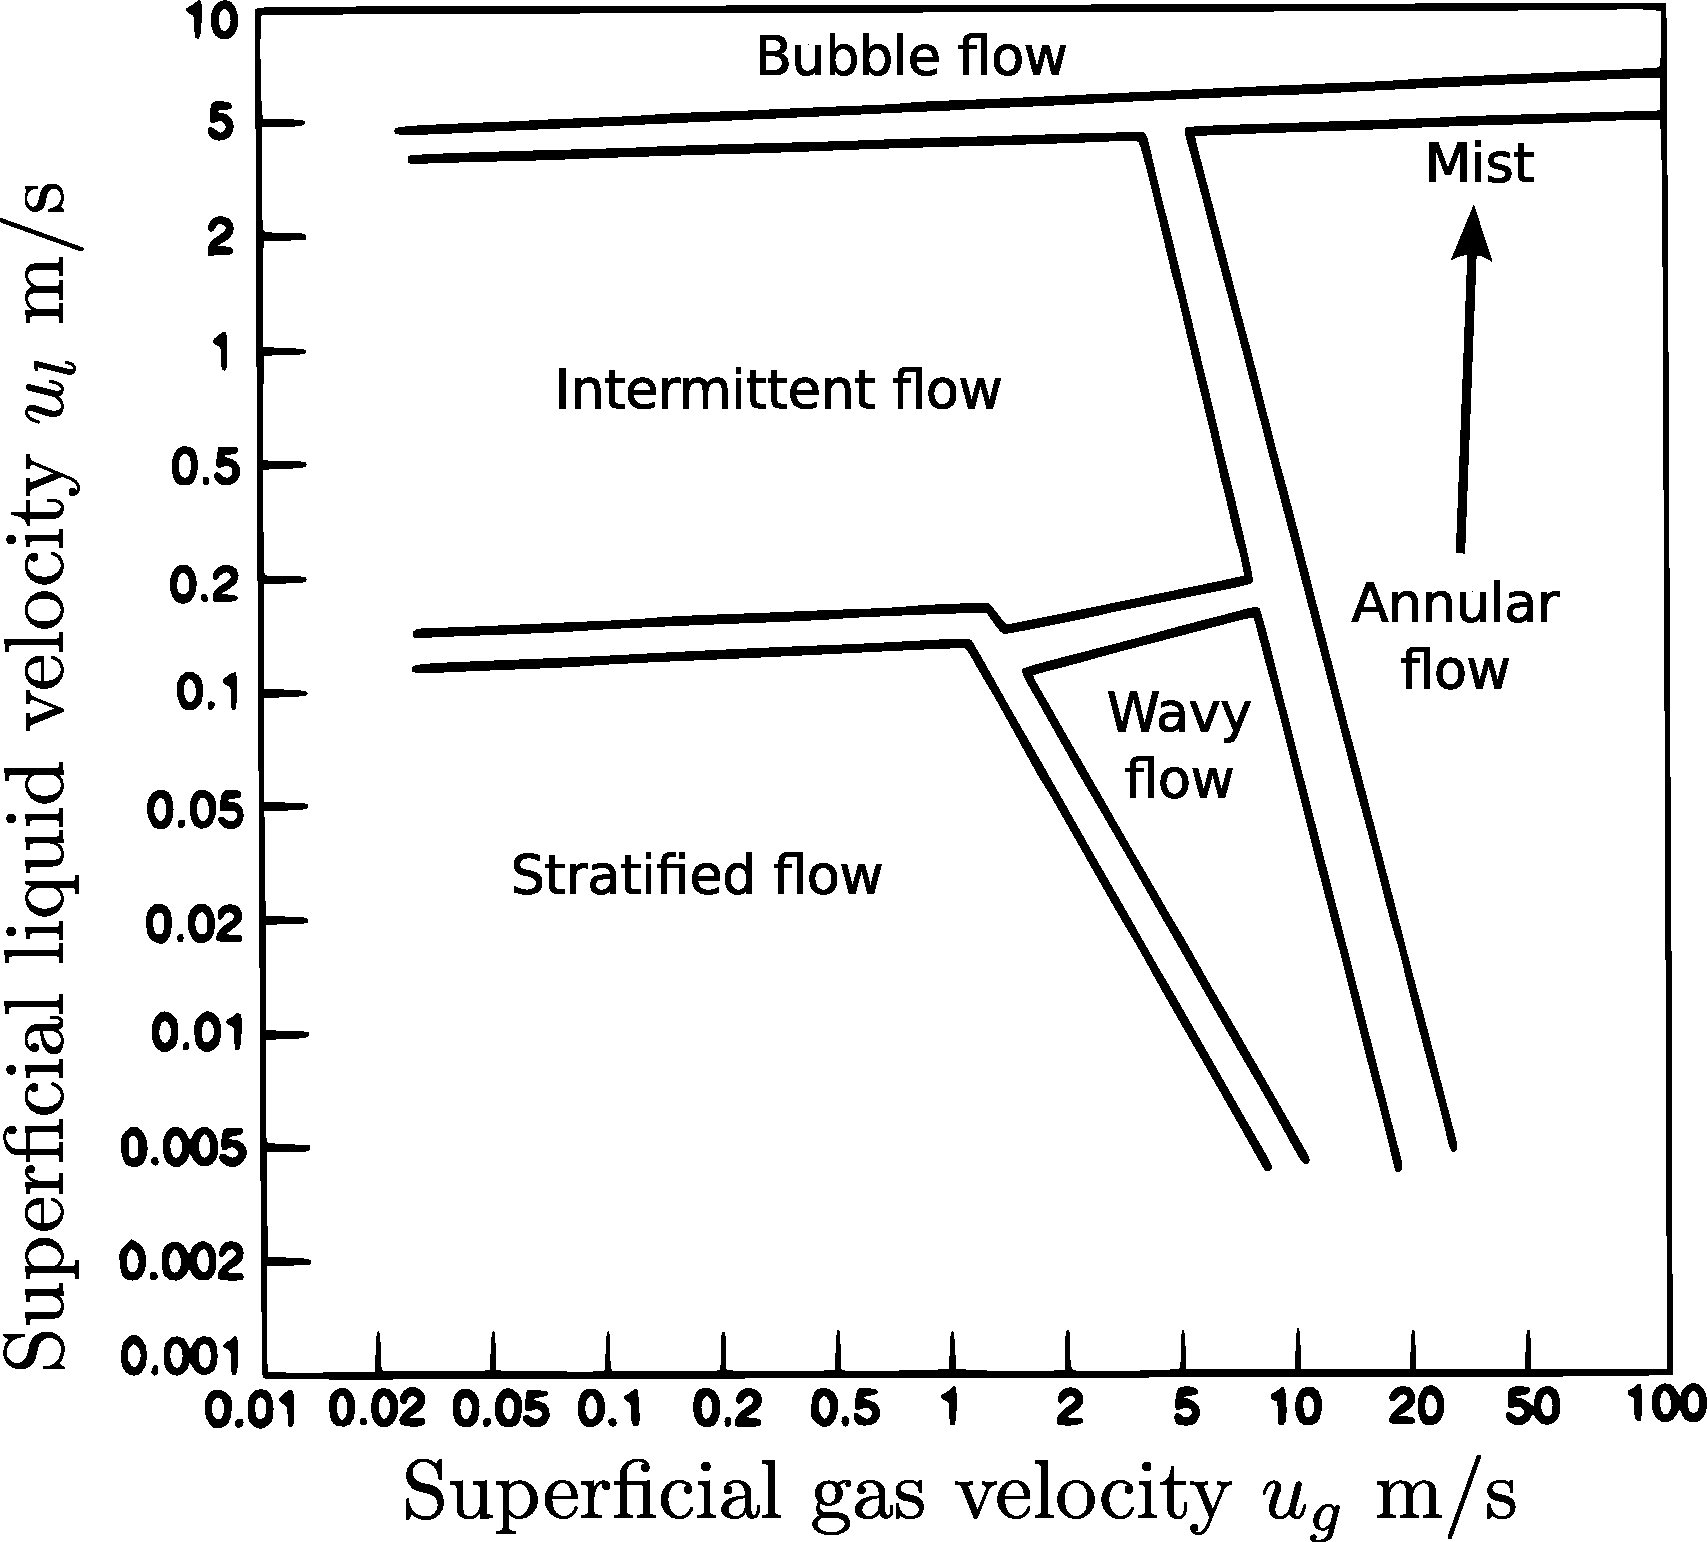
\includegraphics[width=0.65\textwidth,clip]{figures/Chhabra_richardson_flow_map}
  \end{center}
  \caption{Chhabra and Richardson flow pattern map for horizontal pipes.}
\end{figure}

\pagebreak[0]
{\bf Heat Transfer:}\\*
Stefan-Boltzmann constant $\sigma=5.6703\times10^{-8}$~W/m${}^2$~K${}^4$

{\bf Heat Transfer Dimensionless numbers:}
\begin{align*}
  \text{Nu} &= \frac{h\,L}{k} 
  &
  \text{Pr} &= \frac{\mu\,C_p}{k}
  &
  \text{Gr} &= \frac{g\,\beta
    \left(T_w - T_\infty\right)\,L^3}{\nu^2}
\end{align*}

{\bf Resistances}
\begin{align*}
  Q &= U_T\,A_T\,\Delta T = R_T^{-1}\,\Delta T & Q_{rad.}= \sigma\,\varepsilon\,A\left(T_\infty^4-T_w^4\right) = h_{rad.}\,A\left(T_\infty-T_w\right)
\end{align*}
\begin{center}
  \begin{tabular}{|r|c|c|c|c|}\hline
    & \multicolumn{3}{c|}{Conduction Shell Resistances} & Radiation\\
    & Rect. & Cyl. & Sph. & \\\hline
    & & & & \\
    $R$ & $\displaystyle\frac{X}{k\,A}$ & $\displaystyle\frac{\ln\left(R_{outer}/R_{inner}\right)}{2\,\pi\,L\,k}$ & $\displaystyle\frac{R_{inner}^{-1} - R_{outer}^{-1}}{4\,\pi\,k}$ & $\left[A\,\varepsilon\,\sigma\left(T_\infty^2+T_w^2\right)\left(T_\infty + T_w\right)\right]^{-1}$
    \\[5pt]\hline
  \end{tabular}
\end{center}

{\bf Natural Convection}
\begin{table}[h!]
  \begin{center}
    \begin{tabular}{|p{3cm}|p{3cm}|p{3cm}|}\hline
      $\text{Ra}=\text{Gr}\,\text{Pr}$ & $C$ & $m$\\\hline
      $< 10^{4}$ & 1.36 & 1/5\\
      $10^{4}$--$10^{9}$ & 0.59 & 1/4 \\
      $>10^{9}$ & 0.13 & 1/3\\\hline
    \end{tabular}
    \caption{\label{tab:conv}Natural convection coefficients for isothermal vertical
      plates in the empirical relation $\text{Nu}\approx C\left(\text{Gr}\,\text{Pr}\right)^m$.
      % The values are taken from Table~7-1 in ``Heat Transfer'' by J.\
      % P.\ Holman.
    }
  \end{center}
\end{table}

For isothermal vertical cylinders, the above expressions for
isothermal vertical plates may be used but must be scaled by a factor,
$F$:
\begin{align*}
  F = \begin{cases}
    1 & \text{for }\left(D/H\right) < 35\,\text{Gr}^{-1/4}_H
    \\
    1.3\left[H\,D^{-1}\,\text{Gr}_D^{-1}\right]^{1/4}+1 & \text{for }\left(D/H\right) \ge 35\,\text{Gr}^{-1/4}_H
  \end{cases}
\end{align*}
where $D$ is the diameter and $H$ is the height of the cylinder. The
subscript on $\text{Gr}$ indicates which length is to be used as the
critical length to calculate the Grashof number.

Churchill and Chu expression for natural convection from a
horizontal pipe:
\begin{align*}
  \text{Nu}^{1/2} &= 0.6 + 0.387
  \left\{\frac{\text{Gr}\,\text{Pr}}{\left[1 + \left(0.559 /
          \text{Pr}\right)^{9/16}\right]^{16/9}}\right\}^{1/6} &
  \text{for $10^{-5}<\text{Gr}\,\text{Pr}<10^{12}$}
\end{align*}%

{\bf Forced Convection:}\\*
Laminar flows:
\begin{align*}
  \text{Nu} \approx 0.332\,\text{Re}^{1/2}\,\text{Pr}^{1/3}
\end{align*}
Well-Developed turbulent flows in smooth pipes:
\begin{align*}
  \text{Nu} \approx \frac{(C_f/2)
    \text{Re}\,\text{Pr}}{1.07+12.7(C_f/2)^{1/2}\left(\text{Pr}^{2/3}
      -1\right)}\left(\frac{\mu_b}{\mu_w}\right)^{0.14}
\end{align*}

{\bf Boiling:}\\*
Forster-Zuber pool-boiling coefficient:
\begin{align*}
  h_{nb}=0.00122\frac{k_L^{0.79}\, C_{p,L}^{0.45}\, \rho_L^{0.49}}{\gamma^{0.5}\,\mu_L^{0.29}\,h_{fg}^{0.24}\,\rho_G^{0.24}}\left(T_w - T_{sat}\right)^{0.24}\left(p_w-p_{sat}\right)^{0.75}
\end{align*}

Mostinski correlations: 
\begin{align*}
  h_{nb} &= 0.104\,p_c^{0.69}\,q^{0.7}\left[1.8\left(\frac{p}{p_c}\right)^{0.17}+4\left(\frac{p}{p_c}\right)^{1.2}+10\left(\frac{p}{p_c}\right)^{10}\right]\\
  q_c &=
  3.67\times10^4\,p_c\left(\frac{p}{p_c}\right)^{0.35}\left[1-\frac{p}{p_c}\right]^{0.9}
\end{align*}
({\bf Note}: for the Mostinski correlations, the pressures are in units of bar)\\*
{\bf Condensing:}\\*
Horizontal pipes
\begin{align*}
  h = 0.72
  \left(\frac{k^3\,\rho^2\,g_x\,E_{latent}}{D\,\mu\,\left(T_w-T_\infty\right)}\right)^{1/4}
\end{align*}

{\bf Lumped capacitance method:}\\*
\begin{align*}
  \text{Bi} &= \frac{h\,L_c}{\kappa} & \\
  L_c &= 
  V/A & \text{for $\text{Bi}<0.1$}
\end{align*}

{\bf 1-D Transient Heat Conduction:}\\*
\begin{align*}
   Fo = \frac{\alpha \Delta t}{\left(\Delta x\right)^{2}}
\end{align*}


\begin{align*}
   \theta_{\text{wall}} = \frac{T(x,t)-T_{\infty}}{T_{i}-T_{\infty}}= A_{1}e^{-\lambda_{1}^{2}\tau}\cos{\left(\frac{\lambda_{1}x}{L}\right)},\;\;\;\;\; \theta_{\text{cyl}} = \frac{T(r,t)-T_{\infty}}{T_{i}-T_{\infty}}= A_{1}e^{-\lambda_{1}^{2}\tau}\mathbf{J_{0}}\left(\frac{\lambda_{1}r}{r_{0}}\right)
\end{align*}

\begin{align*}
   \theta_{\text{sph}} = \frac{T(r,t)-T_{\infty}}{T_{i}-T_{\infty}}= A_{1}e^{-\lambda_{1}^{2}\tau}\frac{\sin{\left(\frac{\lambda_{1}r}{r_{0}}\right)}}{\frac{\lambda_{1}r}{r_{0}}}
\end{align*}


\begin{align*}
   \left(\frac{\mathcal{Q}}{\mathcal{Q}_{\text{max}}}\right)_{\text{wall}} = 1 - \theta_{0,\text{wall}}\frac{\sin{\lambda_{1}}}{\lambda_{1}},\;\;\left(\frac{\mathcal{Q}}{\mathcal{Q}_{\text{max}}}\right)_{\text{cyl}} = 1- 2\theta_{0,\text{cyl}}\frac{\mathbf{J_{1}}}{\lambda_{1}}
\end{align*}

\begin{align*}
    \left(\frac{\mathcal{Q}}{\mathcal{Q}_{\text{max}}}\right)_{\text{sph}} = 1 - 3\theta_{0,\text{sph}}\frac{\sin{\lambda_{1}}-\lambda_{1}\cos{\lambda_{1}}}{\lambda_{1}^{3}}
\end{align*}

\begin{figure}[h!]%
  \begin{center}%
    \includegraphics[width=0.7\textwidth,clip]{figures/BaselFunctionTable}
  \end{center}
  \caption{Coefficients for the 1D transient equations.}
\end{figure}


\pagebreak[0]

{\bf Overall Heat Transfer Coefficient:}\\*
\begin{align*}
  \dot{\mathcal{Q}} =  \frac{\Delta T}{\mathcal{R}} = U A \Delta T  = U_{i}A_{i}\Delta T = U_{o}A_{o}\Delta T
\end{align*}

\begin{align*}
  \mathcal{R} = R_{i} + R_{\text{wall}} + R_{o} = \frac{1}{h_{i}A_{i}} + \frac{\ln{D_{o}/D_{i}}}{2\pi \kappa L} + \frac{1}{h_{o}A_{o}} 
\end{align*}

{\bf Fouling Factor:}*
\begin{align*}
   \mathcal{R} = \frac{1}{h_{i}A_{i}} + \frac{R_{\text{f,i}}}{A_{i}} + R_{\text{wall}} + \frac{R_{\text{f,o}}}{A_{o}} + \frac{1}{h_{o}A_{o}}
\end{align*}

{\bf LMTD Method:}\\*
\begin{align*}
   \dot{\mathcal{Q}} = U A_{s} \Delta T_{\text{lm}}\;\text{ with }\;  \Delta T_{\text{lm}} = \frac{\left(T_{\text{hot,out}} - T_{\text{cold,out}}\right)-\left(T_{\text{hot,in}} - T_{\text{cold,in}}\right)}{\ln{\left(\frac{T_{\text{hot,out}} - T_{\text{cold,out}}}{T_{\text{hot,in}} - T_{\text{cold,in}}}\right)}}.
\end{align*}

\begin{figure}[h!]%
  \begin{center}%
    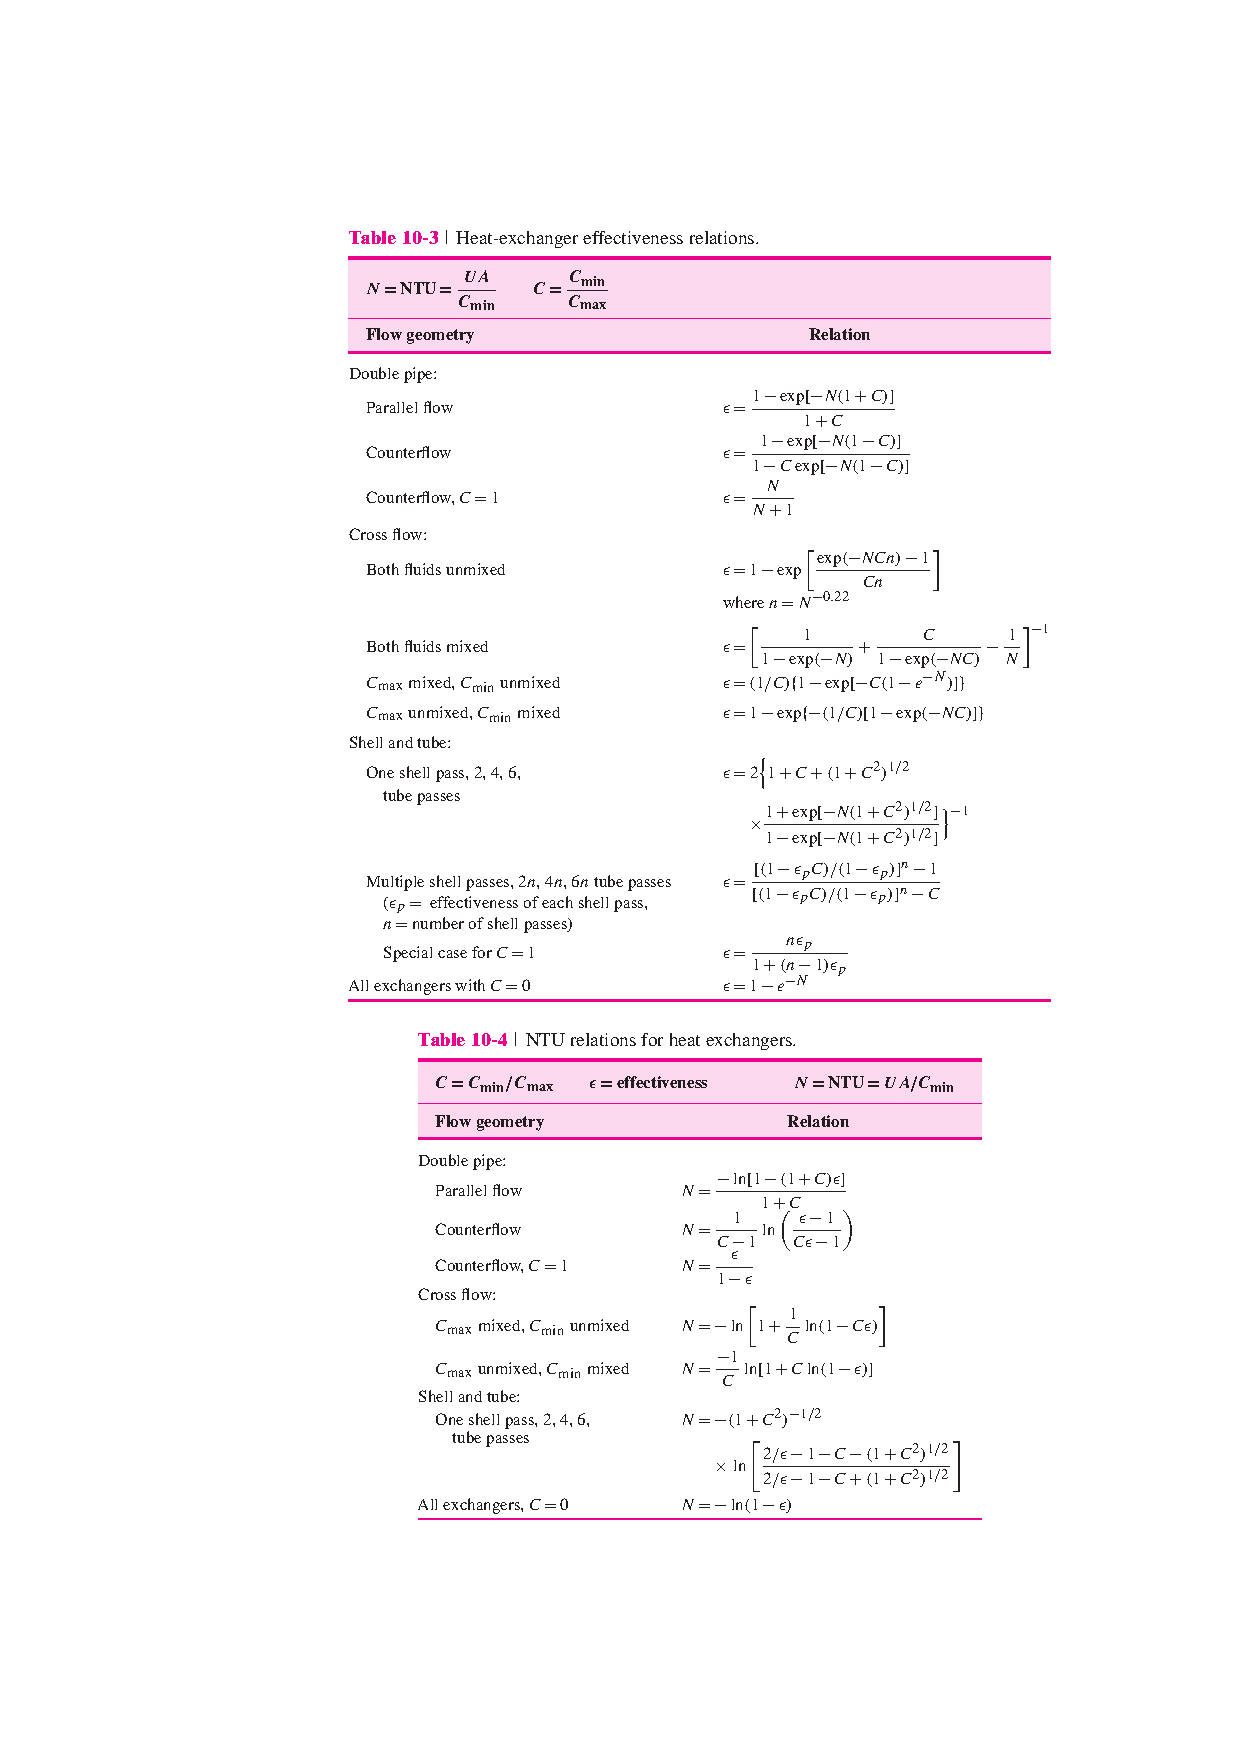
\includegraphics[width=0.8\textwidth,clip]{figures/NTU}
  \end{center}
  \caption{NTU relations}
\end{figure}


\pagebreak[0]
{\bf Diffusion Dimensionless Numbers}\\*
\begin{align*}
  \text{Sc} &= \frac{\mu}{\rho\,D_{AB}} & \text{Le} &= \frac{k}{\rho\,C_p\,D_{AB}}
\end{align*}
\pagebreak[0]
{\bf Diffusion}\\*
General expression for the flux:
\begin{align*}
  \bm{N}_{A} = \bm{J}_A + x_A \sum_B \bm{N}_B
\end{align*}
Fick's law:
\begin{align*}
  \bm{J}_{A} = - D_{AB}\,\nabla C_A
\end{align*}
Stefan's law:
\begin{align*}
  N_{s,r} = -D \frac{c}{1-x}\frac{\partial x}{\partial r}
\end{align*}
{\bf Misc}\\*
\begin{align*}
  P\,V &= n\,R\,T & 
  R&\approx8.314598~\text{J K}^{-1}\text{ mol}^{-1} 
\end{align*}
\end{datasheet}

% \includepdf{BaselFunctionTable.pdf}
\paperend
\end{document}
